% title: 리만 합
% description: 곡선 y = f(x) 아래 [a, b]를 n등분한 직사각형(왼쪽 끝점 기준)으로 넓이를 근사한다. Δx 표시
% packages: pgfplots
% libraries:
% f, a, b, n만 바꾼다. 직사각형 높이: 왼쪽 끝점 {f(x)}, 오른쪽 끝점 {f(x+\dx)}, 중점 {f(x+\dx/2)}.
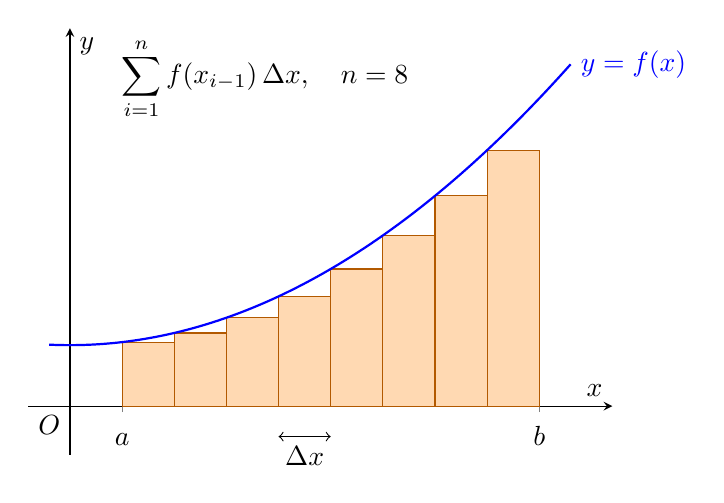
\begin{tikzpicture}[declare function={
    f(\x) = 0.2*\x^2 + 1;
  }]
  \def\a{0.5}
  \def\b{4.5}
  \def\n{8}
  \pgfmathsetmacro{\dx}{(\b-\a)/\n}
  \pgfmathtruncatemacro{\m}{\n+1}
  \begin{axis}[
      width=9cm, height=7cm,
      axis lines=middle, xmin=-0.4, xmax=5.2, ymin=-0.8, ymax=6.2,
      xlabel={$x$}, ylabel={$y$}, xtick={\a,\b}, xticklabels={$a$,$b$}, ytick=\empty,
      typeset ticklabels with strut, clip=false]
    \addplot[ybar interval, fill=orange!30, draw=orange!70!black, samples=\m, domain=\a:\b]
      {f(x)};
    \addplot[thick, blue, domain=-0.2:\b+0.3, samples=100] {f(x)} node[right] {$y=f(x)$};
    \draw[<->] (\a+3*\dx,-0.5) -- node[below] {$\Delta x$} (\a+4*\dx,-0.5);
    \node[anchor=north west] at (0.4,6.2)
      {$\displaystyle\sum_{i=1}^{n} f(x_{i-1})\,\Delta x, \quad n=\n$};
    \node[below left] at (0,0) {$O$};
  \end{axis}
\end{tikzpicture}
